%!TeX root = ../main_buku.tex
%============================================================
% BAB 3: DESAIN SISTEM
%============================================================
\chapter{DESAIN SISTEM}

\section{DESKRIPSI SOLUSI}

Solusi yang diusulkan adalah mengembangkan sistem deteksi dini teks buatan AI pada tugas essay bahasa Inggris mahasiswa yang menggabungkan analisis stilometri dengan pendekatan machine learning. Sistem ini dirancang untuk mengatasi keterbatasan detektor komersial yang tidak mempertimbangkan karakteristik penulis non-native, sekaligus menyediakan antarmuka berbasis web agar dapat digunakan secara praktis oleh dosen maupun mahasiswa. Solusi ini mencakup:
\begin{enumerate}
	\item Modul Ekstraksi Fitur Stilometri yang menganalisis gaya penulisan secara kuantitatif melalui 18 fitur linguistik yang dikategorikan ke dalam empat lapisan (fonologis, morfologis, sintaktis, dan leksikal), sehingga perbedaan pola penulisan manusia dan teks buatan AI dapat direpresentasikan secara numerik.
	\item Model Klasifikasi Random Forest yang dilatih menggunakan fitur stilometri untuk mengklasifikasikan teks sebagai human-written atau AI-generated dengan memanfaatkan mekanisme ensemble dan feature importance yang memungkinkan interpretasi kontribusi setiap fitur terhadap hasil deteksi.
	\item Model BERT yang Di-fine-tune untuk klasifikasi berbasis representasi semantik kontekstual, sehingga sistem dapat menangkap pola linguistik yang tidak terdeteksi oleh fitur stilometri saja.
	\item Antarmuka Aplikasi Web Berbasis FastAPI yang memungkinkan pengguna mengunggah teks essay dan mendapatkan hasil deteksi secara real-time, dilengkapi dengan tampilan skor kepercayaan (confidence score) dari masing-masing model.
	\item Penyimpanan Riwayat Deteksi dengan MySQL yang mencatat setiap hasil analisis beserta metadata teks, sehingga dosen dapat memantau riwayat pengumpulan tugas mahasiswa secara terstruktur.
\end{enumerate}

\section{PERANCANGAN SISTEM}

Alat bantu perancangan yang digunakan untuk menunjang Sistem Deteksi Dini AI-Generated Text pada Tugas Essay Bahasa Inggris Mahasiswa Menggunakan Analisis Stilometri dan Machine Learning adalah Use Case Diagram, Activity Diagram, Class Diagram, dan Entity Relationship Diagram (ERD).

\subsection{Arsitektur sistem}
\begin{figure}[H]
  \centering
  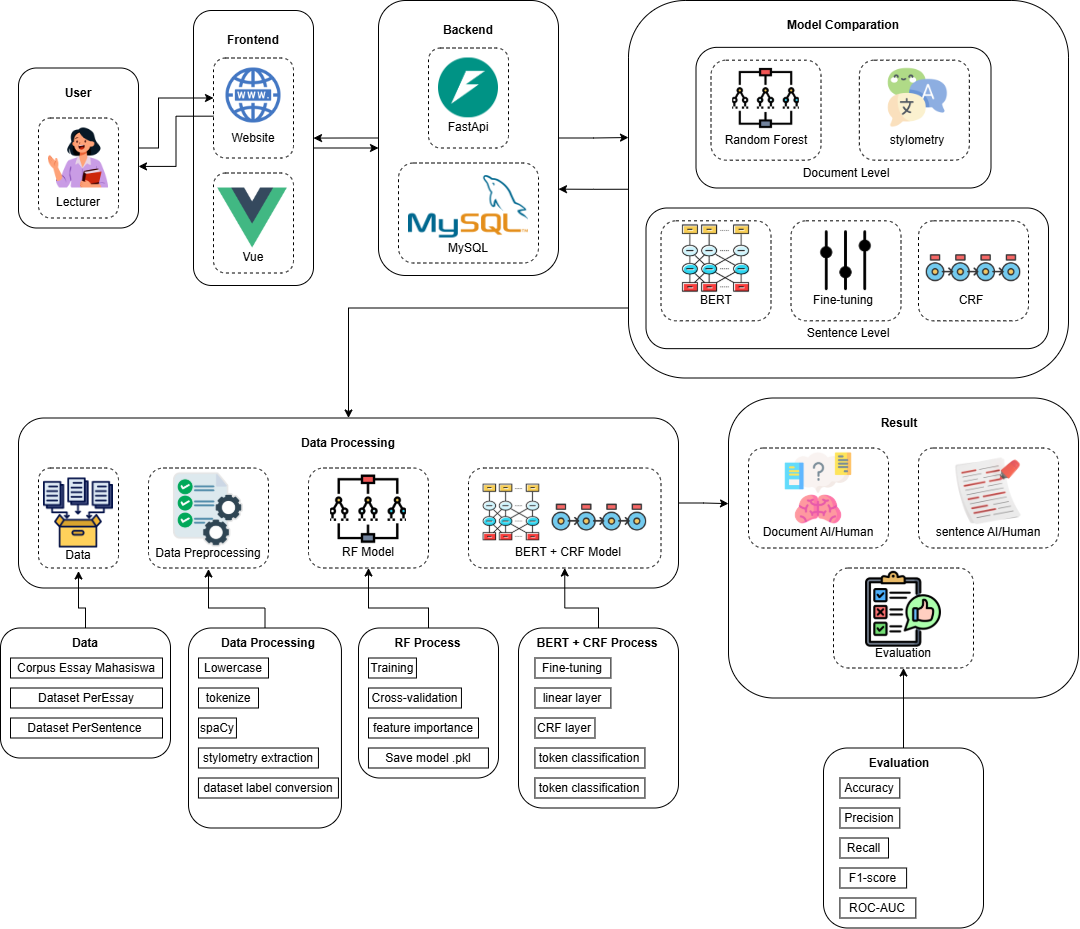
\includegraphics[width=1\textwidth]{assets/diagram/arsitektur_diagram.drawio.png}
  \caption{Diagram Arsitektur Sistem}
  \label{fig:arsitektur_sistem}
\end{figure}

\subsection{Use Case Diagram}

Use Case Diagram merupakan diagram pemodelan dalam Unified Modeling Language (UML) yang bertujuan untuk menggambarkan fungsionalitas perangkat lunak. Diagram ini memetakan interaksi antara aktor (pengguna) dan sistem untuk menjelaskan aktivitas apa saja yang dapat dilakukan dalam aplikasi tersebut.
\begin{figure}[H]
  \centering
  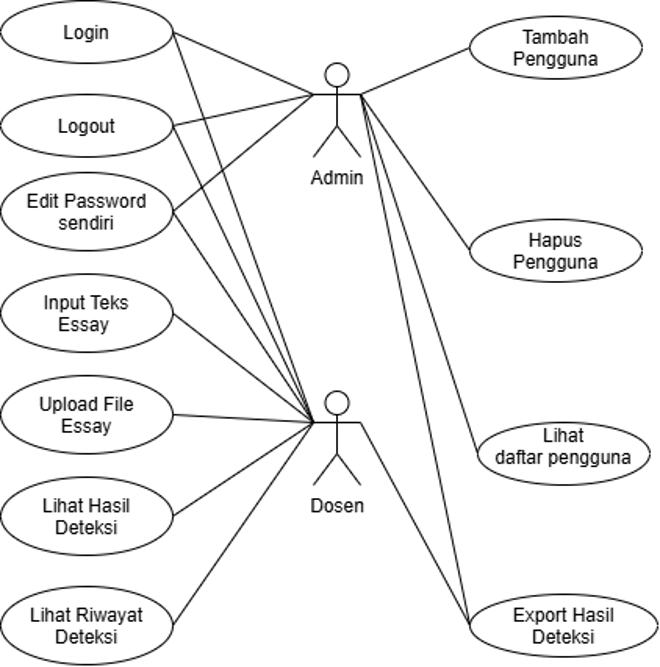
\includegraphics[width=0.8\textwidth]{assets/diagram/use_case.png}
  \caption{Use Case Diagram}
  \label{fig:use_case}
\end{figure}

Penjelasan singkat ini menguraikan fungsionalitas utama berdasarkan aktornya:
\begin{enumerate}[label=\arabic*., leftmargin=*]
  \item Admin: Memiliki hak akses penuh terhadap sistem, mencakup pengelolaan pengguna dan pemantauan seluruh aktivitas deteksi. Fungsi yang dapat dilakukan Admin meliputi:
    \begin{enumerate}[label=\alph*), leftmargin=*]
      \item Login dan Logout.
      \item Edit Password Sendiri.
      \item Manajemen pengguna, meliputi Tambah Pengguna, Hapus Pengguna, dan Lihat Daftar Pengguna.
      \item Export Hasil Deteksi.
    \end{enumerate}
  \item Dosen: Merupakan pengguna operasional yang menggunakan sistem untuk mendeteksi keaslian teks essay mahasiswa. Fungsi yang dapat dilakukan Dosen meliputi:
  \begin{enumerate}[label=\alph*), leftmargin=*]
      \item Login dan Logout.
      \item Edit Password Sendiri.
      \item Input Teks Essay secara langsung maupun Upload File Essay.
      \item Lihat Hasil Deteksi beserta confidence score dari model Random Forest dan BERT.
      \item Lihat Riwayat Deteksi dari pengecekan yang pernah dilakukan.
      \item Export Hasil Deteksi
    \end{enumerate}
\end{enumerate}
